\section{Dizionari e tabelle hash}
I \emph{dizionari} sono una collezione di elementi identificati da una chiave.
Le operazioni che vogliamo poter eseguire sono ricerca, inserimento e cancellazione.
Le possibili implementazioni che abbiamo visto finora sono array e alberi.
Vediamo un riepilogo dei tempi richiesti dalle tre operazioni nelle varie strutture.\\
\begin{tabular}{|l|c|c|c|c|}
    \hline
    \space & \textbf{Array non ord.} & \textbf{Array ord.} & \textbf{Alberi di ricerca} & \textbf{Alberi AVL e 2-3}\\
    \hline
    \textbf{Ricerca} & $\Theta(n)$ & $\Theta(\log n)$ & $\Theta(n)$ & $\Theta(\log n)$\\
    \hline
    \textbf{Inserimento} & $\Theta(1)$ & $\Theta(n)$ & $\Theta(n)$ & $\Theta(\log n)$\\
    \hline
    \textbf{Cancellazione} & $\Theta(n)$ & $\Theta(n)$ & $\Theta(n)$ & $\Theta(\log n)$\\
    \hline
\end{tabular}\\
Non è sempre vero che tenere le cose in ordine ci permette di trovarle più velocemente.
Infatti esistono alcune strutture che disordinano i dati di proposito, ovvero le 
\emph{tabelle hash}.
\subsection{Funzioni hash}
Siano
\begin{itemize}
    \item $U$ = universo delle chiavi
    \item $\lbrace 0 ... m-1\rbrace$ spazio degli indici
\end{itemize}

Funzioni hash h: $U \rightarrow$ $\lbrace 0 ... m-1\rbrace$ trasformazioni di 
chiavi in indici 
\subsection{Fattore di carico}
$\alpha = \frac{n}{m}$\\
\begin{itemize}
    \item $n$ = numero di elementi memorizzati nella tabella
    \item $m$ = posizioni disponibili nella tabella
    \item Se $\alpha$ = 1 la tabella è piena
    \item Se $\alpha$ = 0 la tabella è vuota
\end{itemize}
Quando mi avvicino allo 0 sto "sprecando" la tabella.
Una \emph{funzione hash perfetta (o iniettiva)} è una funzione hash tale che:
\begin{center}
    se $m \neq v \Rightarrow h(m) \neq h(v)$
\end{center}

\noindent Nella pratica, salvo in casi particolari:
\begin{itemize}
    \item Il numero di chiavi possibili è molto più grande del numero di chiavi attese
    \item La dimensione della tabella è scelta paragonabile al numero di chiavi attese
\end{itemize}

\subsection{Gestione delle collisioni}
Supponiamo di voler catalogare 20 persone in una tabella di 26 posizioni e che la nostra
funzione di hash sia la prima lettera del cognome. È una funzione perfetta? No,
perchè esistono lettere più diffuse di altre per i cognomi e rischiamo che due persone vadano a finire nella 
stessa posizione della tabella, creando una \emph{collisione}.
Dobbiamo quindi fare in modo che le collisioni avvengano raramente e, nel caso avvengano,
avere una strategia per gestirle.
Per quanto riguarda il fare in modo che le collisioni avvengano il meno possibile introduciamo i
concetti di \emph{sparpagliamento e uniformità}.
Siano:
\begin{itemize}
    \item h: $U \rightarrow$ $\lbrace 0 ... m-1\rbrace$ una funzione hash
    \item P($x$) la probabilità che scegliendo a caso una chiave da $U$ si scelga $x$
    \item Q($i$) = $\sum_{x | h(x) = i} P(x)$ probabilità che una chiave scelta a caso da $U$
    abbia valore hash $i$
\end{itemize}

\noindent La funzione hash è uniforme se Q($i$) è la stessa per ogni $i$, cioè Q($i$) = $\frac{1}{m}$\\
Alcuni esempi di funzioni hash sono il \emph{metodo della divisione} e il \emph{metodo del ripiegamento}.\\
Esistono due categorie di tecniche per gestire le collisioni: \emph{interne} ed \emph{esterne}.
\subsection{Gestione esterna}
Una tecnica di gestione esterna delle collisioni sono le \emph{liste di collisione}.\\
\begin{figure}[h]
    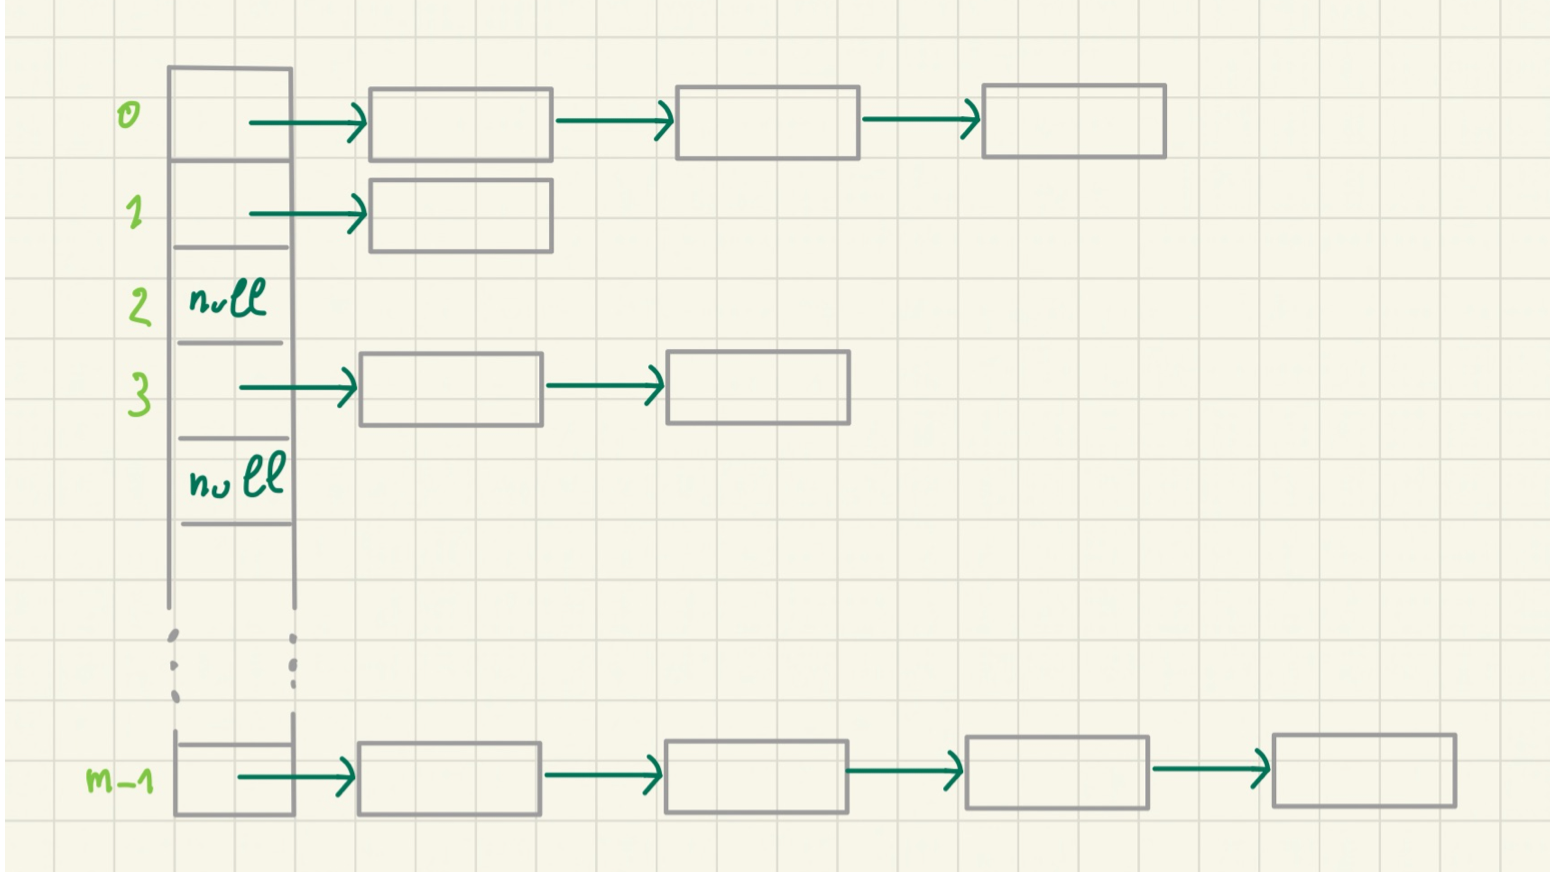
\includegraphics[width=\textwidth]{lista_di_collisione.png}
\end{figure}
\\In posizione $i$ troviamo ogni record la cui chiave $x$ ha valore hash $i$.
La struttura consiste in un array di liste di coppie <elemento, chiave>.
Ogni volta che un nuovo elemento deve essere inserito viene messo esterno alla tabella hash vera e propria
ma collegato alla posizione corretta. Nel momento in cui arriva un nuovo elemento che collide con uno già
presente viene aggiunto alla lista in testa e senza ordinamento.
I tempi delle operazioni sono:
\begin{itemize}
    \item \textbf{Inserimento}: $O(1)$
    \item \textbf{Ricerca}: $O(m)$
    \item \textbf{Cancellazione}: $O(n)$
\end{itemize}
Il tempo medio è $O(1+\alpha)$, dipende dalla lunghezza della lista.\\
Quando una lista si riempie troppo si parla di \emph{agglomerazione} ed è un problema che dobbiamo cercare di evitare.
Se si verifica significa che la funzione scelta non è adeguata dal punto di vista dell'uniformità.

\subsection{Gestione interna}
Esistono diverse metodologie interne per la gestione delle collisioni. Vedremo l'indirizzamento aperto.
A grandi linee, possiamo dire che memorizziamo tutto nella tabella e in caso
di collisione troviamo un altro posto libero scegliendo una delle possibili strategie.
La prima strategia è cercare il primo posto vuoto disponibile e se arrivo in fondo
riparto dalla cima. Questo sistema è afflitto dal tipo peggiore di agglomerazione, detta agglomerazione
primaria, che si verifica quando ho valori con chiavi di diversi valori di hash che si mescolano.
Formalmente questa metodologia si chiama \emph{funzione ausiliaria},
nello specifico \emph{scansione lineare} $C(k,i)$, dove 
$k$ è la chiave, $i \ge 0$, $C(k,i) = (h(k)+i) \mod{m}$.

\subsubsection{Scansione quadratica}
$C(k,i) = \lfloor h(k)+C_{1}i+C_{2}i^2 \rfloor \mod{m}$\\
Questa funzione ausiliaria ci permette di evitare l'agglomerazione primaria ma non interviene su
quella secondaria (meno grave ma comunque fastidiosa).

\subsubsection{Hashing doppio}
$C(k,i) = [h(k)+ih'(k)] \mod{m}$ dove $h'$ è una seconda funzione hash.
La situazione ideale sarebbe $h(k_{1}) = h(k_2) \Rightarrow h'(k_{1}) \neq h'(k_2)$\\
In parole povere significa che se trovo un posto occupato provo ad usare una differente
funzione (la stessa cosa con l'incremento di $i$).

\subsubsection{Operazioni}

\begin{algorithm}
    \caption{Inserimento di un elemento nella tabella}
    \Indm\textbf{Algoritmo} \emph{inserimento(elemento i, chiave k)}\\
    \Indp$i \leftarrow 0$\\
    \While{$i < m$ \textbf{and} $v[C(k,i)]$ è occupata}{
        $i \leftarrow i + 1$
    }
    \eIf{$i < m$}{
        $v[C(k,i)] \leftarrow (e.k)$
    } {
        errore! tabella piena
    }
\end{algorithm}

\begin{algorithm}
    \caption{Ricerca di un elemento nella tabella}
    \Indm\textbf{Algoritmo} \emph{ricerca(chiave k)} $\rightarrow$ \emph{elemento}\\
    \Indp$i \leftarrow 0$\\
    \While{$i < m$ \textbf{and} $v[C(k,i)]$ è occupata \textbf{and} $v[C(k,i)].chiave \neq k$}{
        $i \leftarrow i + 1$
    }
    \eIf{$i = m$ \textbf{or} $v[C(k,i)]$ è libera}{
        \Return{null}
    } {
        \Return{$v[C(k,i)].elemento$}
    }
\end{algorithm}
Per quanto riguarda la cancellazione, questa è più insidiosa perchè, ogni volta che si cancella un
elemento, andrebbe ristrutturata la tabella, in quanto si perderebbero i legami impliciti
tra le celle che vengono usati nelle ricerche. Per questo motivo non avviene mai 
una cancellazione vera e propria ma una "virtuale": introduciamo un flag booleano
che indichi se il dato contenuto in quella posizione è cancellato o meno. Quando ci sarà 
un nuovo inserimento il dato vecchio sarà sovrascritto e il flag riportato a "non cancellato".

\subsubsection{Numero di confronti}
\begin{tabular}{|l|c|c|}
    \hline
    \space & \textbf{Scansione lineare} & \textbf{Scansione quadratica e hashing doppio}\\
    \hline
    \textbf{Chiave trovata} & $\frac{1}{2} + \frac{1}{2(1-\alpha)}$ & $\frac{1}{\alpha} \log \log_2(1-\alpha)$\\
    \hline
    \textbf{Chiave non trovata} & $\frac{1}{2} + \frac{1}{2(1-\alpha)^2}$ & $\frac{1}{1-\alpha}$\\
    \hline
\end{tabular}\\
Ricordiamo che $\alpha$ è il fattore di carico della tabella.
Se $\alpha < 1$ i confronti saranno sempre in numero molto limitato.
Questo significa che le funzioni ausiliarie da noi esposte sono efficienti più la tabella è vuota.
Questa considerazione ci porterà alla ricerca di alcuni metodi (\emph{re-hashing}) atti 
al mantenimento di un minimo di posti liberi ridimensionando la tabella.
\subsubsection{Re-hashing}
Si tratta della sostituzione della tabella con una nuova.
È un'operazione molto dispendiosa in termini di tempo. Occorre inoltre una funzione hash adatta alla nuova tabella.
Per quanto riguarda lo spostamento degli elementi dalla tabella vecchia a quella nuova occorre scandire l'intera tabella
e inserire ogni suo elemento nella nuova tabella,
calcolandone la posizione in base alla nuova funzione di hash e risolvendo eventuali collisioni.
Pertanto il re-hashing richiede un numero minimo di passi pari almeno alla dimensione della vecchia tabella.
Sebbene appaia molto dispendioso in termini di tempo, se gestito bene ha un costo 
ammortizzato basso. Supponiamo di procedere come segue:
\begin{itemize}
    \item Fissiamo il valore massimo del fattore di carico ad $\alpha_{max} = \frac{1}{2}$
    \item Ogni volta che il fattore di carico raggiunge il valore massimo al 
    momento del successivo inserimento effettueremo il re-hashing sostituendo la tabella con una nuova 
    di capacità doppia.
\end{itemize}
Immaginiamo di avere una tabella $T_0$ di dimensione $m$ e di effettuare una serie 
di inserimenti, sostituendo, quando necessario, una tabella $T_i$ con una tabella $T_i+1$ mediante re-hashing.
\begin{figure}[h]
    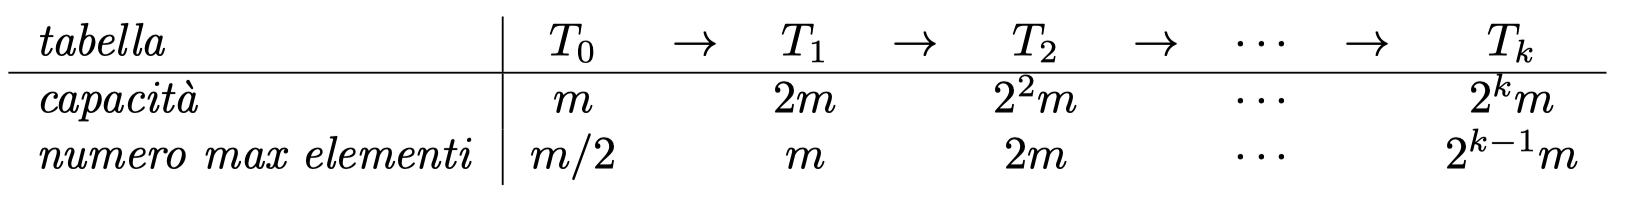
\includegraphics[width=\textwidth]{rehashing.png}
\end{figure}
Il numero totale di operazioni di inserimento che si effettuano a causa dei re-hashing è
$\frac{m}{2}(2^{k} - 1)$\\
Possiamo concludere che se efffettuiamo $N$ operazioni di inserimento in una 
tabella hash, a causa del re-hashing effettuiamo in totale $O(N)$ ulteriori inserimenti.
Se ogni operazione di inserimento utilizza un numero di passi costante, il numero di passi totali tenendo conto anche 
del re-hashing è $O(n)$. Pertanto, dividendo per il numero $N$ di inserimenti "effettivi", otteniamo
che il tempo ammortizzato è $\frac{O(n)}{N} = O(1)$. Quindi, anche effettuando il re-hashing 
nel modo indicato sopra, il costo medio delle operazioni di inserimento resta costante.
\clearpage